% ---------------------------------------------------------------------------------------
% ---------------------------------------------------------------------------------------
% Specifications
% ---------------------------------------------------------------------------------------
% ---------------------------------------------------------------------------------------

\documentclass[12pt]{article}
\usepackage[letterpaper, margin=1in]{geometry}
\usepackage{newtxtext,newtxmath}
\usepackage[math-style=ISO]{unicode-math}
\usepackage{fullpage}
\usepackage[authoryear,sectionbib]{natbib}
\linespread{1.7}
\usepackage[utf8]{inputenc}
\usepackage{lineno}
\usepackage{titlesec}
\titleformat{\section}[block]{\Large\bfseries\filcenter}{\thesection}{1em}{}
\titleformat{\subsection}[block]{\Large\itshape\filcenter}{\thesubsection}{1em}{}
\titleformat{\subsubsection}[block]{\large\itshape}{\thesubsubsection}{1em}{}
\titleformat{\paragraph}[runin]{\itshape}{\theparagraph}{1em}{}[. ]
\renewcommand{\refname}{Literature Cited}
\DeclareTextSymbolDefault{\dh}{T1}
\medmuskip=8mu 
\thickmuskip=10mu
\usepackage{graphicx}
\usepackage{booktabs}
\renewcommand{\thetable}{\Roman{table}}
\usepackage{caption}
\captionsetup{justification = raggedright,
              singlelinecheck = false,
              labelfont = bf}






% ---------------------------------------------------------------------------------------
% ---------------------------------------------------------------------------------------
% Title page
% ---------------------------------------------------------------------------------------
% ---------------------------------------------------------------------------------------

\title{Photosynthesis-light relationships are more variable in time than in space 
        for a shallow eutrophic lake}

\author{
Joseph S. Phillips$^{1,2,\dagger}$ \\
Amanda R. McCormick$^{1,3}$ \\
Jamieson C. Botsch$^{1}$ \\
Kristian R. Book$^{1}$ \\
Anthony R. Ives$^{1}$}

\usepackage{amsmath} % for split math environment

\date{}

\begin{document}

\raggedright
\setlength\parindent{0.25in}

\maketitle

\noindent{} 1. Department of Integrative Biology, University of Wisconsin, Madison, Wisconsin 53706 USA

\noindent{} 2. Department of Aquaculture and Fish Biology, H\'{o}lar University, Skagafj\"{o}r{\dh}ur 551 Iceland

\noindent{} 3. Department of Land, Air and Water Resources, 
University of California, Davis, CA, USA

\noindent{} $\dagger$ E-mail: joseph@holar.is

\bigskip

Running head: {Variable PI curves}

\linenumbers{}

\clearpage





% ---------------------------------------------------------------------------------------
% ---------------------------------------------------------------------------------------
% Abstract
% ---------------------------------------------------------------------------------------
% ---------------------------------------------------------------------------------------

% \bigskip
% 
% \textit{Keywords}: {}
% 
% \clearpage





% ---------------------------------------------------------------------------------------
% ---------------------------------------------------------------------------------------
% Introduction
% ---------------------------------------------------------------------------------------
% ---------------------------------------------------------------------------------------

\section*{Background}

The data described here are from ``light gradient incubations'' 
conducted at M\'{y}vatn in in 2018 and 2019. 
Pelagic and benthic incubations were conducted at ST33 and Reykjahli{\dh} in 2018
and at those two locations plus E5 in 2019. 
Here, I treat ST33 as reprsentative of the South Basin,
Reykjahli{\dh} as representative of the North Basin,
and E5 as representative of the East Basin.
In both years, there were substantial cyanobacteria blooms; 
it will probably be good to present data on spatiotemporal patterns in the blooms.
In 2018, we collected data in June, July, and August;
while in 2019 we only collected data in July and August.
For a given year-month combination, 
sampling events across sites and zone (pelagic vs. benthic)
were either conducted on the same day or within a few days.
Note that some combinations of sample date, basin, 
and zone (benthic vs. pelagic) are missing.

Benthic incubations used intact sediment cores in the tall acrylic tubes,
while pelagic incubations used water collected with the Schindler trap in the short tubes.
Schindler tows were taken for the full water column depth at a given site
to provided an integrated picture of the full water column.
We wrapped tubes with varying layers of mosquito net or black plastic 
to create a gradient of light levels. 
For the benthci incubations, we also wrapped the bottom portion of each tube 
corresponding to the sediment layer with black plastic.

We conducted incubations using floating racks, with the tubes hanging at 0.5m 
following the routine incubations.
After setting up the racks and shading, we allowed the tubes to acclimate for about 1h
befor taking the initial DO readings. 
After the initial readings, the tubes were incubated
for an average of either 6.24h (min = 3.48h; max 8.83h) for the pelagic
or 1.99h (min = 1.05h; max 3.33h) for the benthic.
I calculated the net metabolism in each tube as the change in DO concentration 
(converted to mg $\text{m}^{-3}$), multiplied by the water column depth, 
and divided by the incubation duration.
This resulted in areal flux rates, 
which can be interpreted as DO fluxes across either the sediment surface (for the benthic)
or across an average water-column cross-section (for the pelagic). 
The benthic and pelagic data are comparable as aeral flux rates, 
although comparting total benthic vs. pelagic production would require
integrating the pelagic fluxes across the full water column depth.

The ambient light environment during the incubations was quantified 
using combination of Li-COR readings taken multiple times during each incubation
and HOBO loggers deployed on the racks (when available).
The light available in the tubes was estimated based on the number of layers of mosquito net,
for which we determined a fixed conversion using the Li-COR meter in empty acrylic tubes
with the corresponding amount of shading and with the top stoppered.

Some additional data were taken, 
including midges (tube counts and larvaal form sieved sediment) 
and chlorophyll/phycocyanin from handheld probes and from filtration. 
However, these data have some gaps and there are some weird anamolies in the chlorophyll data
(e.g., the hanheld and filtered measurements are not correlated, 
even though we have independent confirmation from other data that they should be).
Therefore, I am not currently including those data in any analyses.





% ---------------------------------------------------------------------------------------
% ---------------------------------------------------------------------------------------
% Methods
% ---------------------------------------------------------------------------------------
% ---------------------------------------------------------------------------------------


\section*{Fitting the PI curves}

I fit a single model to the data for all sites and sampling dates, 
done separately for the benthic and pelagic data.
While I fit the two zones separately, 
I wanted to use a PI curve of the same form 
so that the parameter estimates would be comparable.
The pelagic incubations showed clear signs of photoinhibition,
while the benthic did not. 
Therefore, I fit the data with a two-parameter photoinhibition curve 
(plus a parameter for respiration):
%
\begin{equation} \label{eq:pi-curve}
    \text{NEP}_i = \beta_{s(i)} \times \left(\frac{\text{PAR}_i}{\omega_{s(i)}} \right) 
                    \times \text{exp} \left(1 - \frac{\text{PAR}_i}{\omega_{s(i)}} \right)
                      - \rho_{s(i)} + \epsilon_i
\end{equation}
%
where $\beta_{s(i)}$ is the maximum GPP, 
$\omega_{s(i)}$ is the optimum PAR, 
$\rho_{s(i)}$ is respiration,
and $\epsilon_i$ is a residual for observation $i$.
The function $s(i)$ maps observations to date-site combination $j$,
such that a single PI curve is inferred for each.

The optimum PAR $\omega_j$ scales the rate at which the maximum GPP is reached
(with higher $\omega_j$ corresopnding to a slower saturation).
This can be illustrated by calculating the initial slope of the PI curve 
(i.e., ``$\alpha$'' in the hyperbolic-tangent model):
%
\begin{equation} \label{eq:alpha}
    \alpha = \lim_{\text{PAR}\to 0} \frac{\text{d}\text{NEP}_j}{\text{d}\text{PAR}} = 
        e \times \frac{\beta_j}{\omega_j}.
\end{equation}
%
where $e$ is base of the natural logarithm.
An important corollary of this point is that $\omega_j$ is a meaningful parameter
even if the observed PAR remains well below the optimum PAR.
An alternative would be to parameterize the model in terms of $\alpha$ 
and interpret the results in terms of this initial slope. 
However, the reparameterized version makes the overall form of the curve 
(and specifically $\beta_j$ as the max GPP) less clear.
I also like that $\omega_j$ has units of PAR, 
which makes it easier to interpret its scale.
Below I discuss how this can be related to the half-saturation constant to help 
compare my PI curve fits to Amanda's \textit{Inland Waters} paper.

Variation in $\beta_j$ was modeled as
%
\begin{equation} \label{eq:random}
    \beta_{j} \sim \text{lognormal} \left(\mu_{\beta},~\sigma_{\beta}\right)
\end{equation}
%
where $\mu_{\beta}$ is the mean and $\sigma_{\beta}$ is the standard deviation 
on the log scale.
Variation in $\omega_j$ and $\rho_j$ was modeled analagously,
with parameters $\mu_{\omega}$  
and $\sigma_{\omega}$ for the former; 
and $\mu_{\rho\right}$ 
and $\sigma_{\rho}$ for the latter.
The lognormal variaion in $\beta_j$ (for example) can also be expressed as 
$\beta_{j} = e^{\mu_{\beta}} \times e^{\sigma_{\beta}Z_j}$
where $Z_j$ is a standard-normal deviate.
This illustrates that the standard deviaitons characterize proportional changes
with respect to some reference scale (i.e., $e^{\mu_{\beta}}$)
and therefore are directly comparable across different parameters,
despite the fact that $\omega_j$ has different units than $\beta_j$ and $\rho_j$
(also note the data standardization discussed next).

I z-scored the aeral DO flux data and divided PAR by its mean across the full data set 
for each zone prior to fitting the model. 
I then back-scaled the parameters accordingly.
I fit the models using Bayesian approach in Stan 2.19,
run in R 4.0.3 usin the \texttt{rstan} package.
The model was fit with 4 chains,
3000 iterations (1500 of warm-up and 150 of sampling),
tree depth of 11, and ``adapt delta'' of 0.975.
Convergence was assessed by the number of divergent transitions 
and the potential scale reduction factor (\^{R}),
which quantifies the relative variance within and between chains. 
We used posterior medians as point estimates
and quantile-based uncertainty intervals
with coverage analogous to standard errors
(16\% and 84\% quantiles for 68\% coverage).
The model used standard-normal priors for the means of the lognormal distributions
and Gamma priors with 1.5 and scale parameter 0.75 for all standard deviations.

To futher characterize patterns of spatial and temporal variation in the PI curves,
I calculated pairwise correlations between $\beta_{j}$, $\omega_j$, and $\rho_j$ 
across date-site combinations.
I did this separately for benthic nad pelagic production. 
To quantify the relative variation among sites and among sampling dates (i.e., within sites),
I used ANOVA to calculate F ratios of between vs. within site variation
in $\beta_j$, $\omega_j$, and $\rho_j$.
For both the correlations and the F-tests I used the parameter estimates on the
log scale, because they were more symmetrically distributed.
Moreoever, I report the F ratios themselves on the log-scale, 
since they are symmetrical about 0;
log F-ratio > 0 indicates greater variance between sites,
while a log F-ratio < 0 indicates greater between sampling dates (i.e., within sites).
I performed these calculations across the full posterior distributions for the parameters,
resulting in posterior distributions of correelations and of log F-ratios.




% ---------------------------------------------------------------------------------------
% ---------------------------------------------------------------------------------------
% Results
% ---------------------------------------------------------------------------------------
% ---------------------------------------------------------------------------------------

\section*{Results}

The photoinhibition model fit both the pelagic and benthic data well
(Figures \ref{fig:nep-pel} and \ref{fig:nep-ben}).
Benthic GPP was clearly detected for all date-site combintions,
while for several dates in both the North and South basins GPP was very low
across all light levels.
For those date-site combinations that did have substantial pelagic GPP,
there was evidence of modest photoinhibition.
In contrast, benthic GPP did not appear to be photoinhibited on any sample dates.

For the pelagic PI curves, 
maximum GPP varied substantially through time in both the North and South basins 
(Figures \ref{fig:par} and \ref{fig:sd}),
broadly corresponding to increases in water-column cyanobactera 
[data not shown, but it would be good to do so I think].
However, pelagic optimum PAR and respiration were very similar between basins
and remained quite stable through time.
Furthermore, these parameters were not correlated across sample events,
suggesting that the large temporal variability in maximum GPP
did not lead to changes in the other parameters.
This is perhaps not too suprising for optimum PAR,
although we would expect respiration to increase with GPP if both 
are coupled to algal biomass. 
This suggests that much of the pelagic respiration is due to heterotrophic organisms,
such as zooplankton or bacteria.

For the benthic PI curves,
maximum GPP only modestly varied through time and between basins 
(Figures \ref{fig:par} and \ref{fig:sd}).
The largest spatial contrast was between the North and South basins 
in June of 2018, 
and the largest within-basin temporal contrast was for the South basin
between June and August of 2018.
Optimum PAR was also quite consistent across date-site combinations,
except for the large increase in the East Basin in August 2019.
This can be seen directly in Figure \ref{fig:nep-ben},
with a very gradual increase in net production across a wide range of light levels
[note these were high because the water was clear and it was a sunny day].
In 2018, benthic respiration was quite similar between the North and South basins 
and varied little through time. 
This remained true in the beginning of 2019, 
however in August benthic respiraion substantially increased in the North and East basins.
This inferred increaase in respiration can be directly seen in the low DO flux values
at low light levels in Figure \ref{fig:nep-ben}.
Similar to pelagic production, optimum PAR was not correlated with maximum GPP and respiration in the benthos (Table \ref{tab:cor}).
However, maximum GPP and respiration were strongly correlated,
reflecting both spatial and temporal patterns visible in Figure \ref{fig:par}.
This coupling of maximum GPP and respiration is consistent with benthic primary producers
being major direct contributors to respiration. 
However, it is also possible that heterotrophic respiration increase 
through utilization of the increased primary primary production.
It also worth noting that variation in respiration was greater than for maximum GPP,
suggesting that processes not coupled to primary production contributed 
to variation in benthic respiration.

The log F-ratios were broadly near zero, 
indicating that variation among between sites and between sample dates was broadly similar
(Figure \ref{fig:var}).
However, nearly all of the log F-ratios were less than zero, 
with the lone exception of benthic optimum PAR.
Therefore, variaion among sampling dates was generally larger than variation among sites.
Moreover, the two F ratios most clearly below zero, pelagic max GPP and benthic respiration,
corresponded to the two parameters with the greatest overall level of variability 
(Figure \ref{fig:sd}).
Together, these results indicate that while variation in benthic and pelagic PI curves
was comparable in time and space, variation in time predominated. 




\section*{Comparison to previous results}

In this analysis, temporal variation in primary production (and particularly maximum GPP)
was much higher for pelagic production than for benthic relative to their respective scales.
Of course, benthic production is greater on an aeral basis, 
and this is probably still true if integrating pelagic production across the water column
(as Amanda found in the \textit{Inland Waters} paper).
So it might be that the variation in overall production due 
to benthic photosynthesis is larger than the pelagic contribution.
Nonethless, this result does remind me of my \textit{L\&O} paper,
where maximum GPP was the dominant contributor to variation in overall GPP
and was pretty closely correleated to water column phycocyannin.
Amanda also found that pelagic production can exceed benthic production 
when pelagic biomass is sufficiently high to supress benthic production 
through light limitation.
So, increases in phytoplankton biomass may still be a major contributor to 
variation in total GPP via changes in max GPP and shading of the benthos.

Another way to approach this issue is to directly compare the estimtaes of 
maximum GPP between this study and Amanda's.
It is worthing pointing out that Amanda's esimtates of pelagic max GPP
used some of the same incubations as I used here. 
In contrast, the benthic incubations used entirely distinct data,
since Amanda used the routine Sttaion 33 incubations.
The overall magnitude and variability of benthic max GPP in 2018
was similar between Amanda's paper (Fig. 4).
However, according to Amada's paper benthic max GPP was somewhat unusual in 2018 
in being so low and temporally consistent.
My estimtes suggest that 2019 continued the pattern from 2018.
If max GPP in 2020 and 2021 was also low, 
perhaps that could serve as an indictor for an immending midge crash. 
If midges are surviving on "old" organic material,
perhaps it take several years of low benthic production to 
lead to sufficient depletion of of organic material to allow them to start crashing.
Amanda's esimtates of pelagic max GPP are a little harder to see in Fig. 4 of her paper,
but they seem not to increase as much as my estimates. 
Since they are the same data, this is probably because her estimates 
coutple max GPP to estimates of chlorophyll, 
so variation in max GPP not associated with chlorophyll would not be captured.

I think these comparisons to Amanda's results underscore the value of the routine incubation
data across so many years, since there is a lot of variation in max GPP one would miss
if only using 1-2 years as is the case for my analysis.
That said, I think this actually reinforces the main finding of my analysis.
Even across two years with comparatively limited variation in max GPP 
(judged by comparison to Amanda's paper) 
and capturing the widest spatial scale of variation possible within M\'{y}vatn 
(contrasts between basins) 
temporal vaariation is still at least as large if not larger than spatial variation.
And this is true for both benthic and pelagic production,
despite the sense that the North Basin is ``bloomier'' than the South 
(though this is obviously an over simplification).

So far, I've focused on max GPP. 
But I think it is also interesting to consider sensitivity to light variation.
The photoinhibition model is parameterized in terms of optimum PAR 
(reproduced here dropping indexing and respiration):
%
\begin{equation} \label{eq:pi-curve-simp}
    \text{NEP} = \beta \times 
                  \left(\frac{\text{PAR}}{\omega} \right) 
                    \times \text{exp} \left(1 - \frac{\text{PAR}}{\omega} \right).
\end{equation}
%
In my \textit{L\&O} paper, I found that the initial slope of the PI curve varied 
quite dramatically through time, and this was negatively correlated with light.
this led to the suggestion that there was acclimation to light limitation.
In the present analysis, I found that optimum PAR did not vary much for either pelagic or benthic production.
However, the slope of the PI curve for the photoinhibition model is proportional (either directly or inversely) to both $\beta$ and the $\omega$ (equation \ref{eq:alpha}).
Pelagic $\beta$ was quite variable, 
and this would translate to large variation in $\alpha$.
So, this result seem consistent.

In Amanda's \textit{Inland Waters} paper, she used a Michaelis-Menten curve:
%
\begin{equation} \label{eq:mm-curve}
    \text{NEP} = \frac{\beta~\text{PAR}}{K + \text{PAR}}
\end{equation}
%
where $\beta$ has the same interpretion as the maximum GPP 
and $K_{\text{MM}$ is the half-saturation constant.
An expresson for the half-saturation level for the photoinhibition model 
can be obtained by solving the equation 
%
\begin{equation} \label{eq:half-sat-exp}
    \left(\frac{K}{\omega} \right) 
                    \times \text{exp} \left(1 - \frac{K}{\omega} \right) 
                    = 0.5
\end{equation}
%
for $K$ when $0 < K < \omega$, which yields
%
\begin{equation} \label{eq:half-sat-sol}
    K = -\omega~W\left(-0.5/e\right)
\end{equation}
%
where $W$ is the product log function. 
This cannot be expressed in terms of elementary functions,
but approximately evaluates as 
%
\begin{equation} \label{eq:half-sat-num}
    K \approx 0.231961~\omega
\end{equation}
%
Amanda estimated pelagic and benthic half-saturation as
$K$=46 $\mu\text{mol}~\text{photons}~\text{m}^{-2}~\text{s}^{-1}$
and
$K$=111 $\mu\text{mol}~\text{photons}~\text{m}^{-2}~\text{s}^{-1}$,
respectively.
These are very close to my estimates based on the average $\omega$:
$K$=45 and $K$=104 $\mu\text{mol}~\text{photons}~\text{m}^{-2}~\text{s}^{-1}$, 
for benthic and pelagic, respectively.
I think this suggests that the routine incubations provide pretty decent estimates 
of PI curve parameters,
altough this depends on a wide range of PARs that comes with many sampling events.

Largely as an aside, I was curious about how close the photoinhibition model 
is to the Michaelis-Mention and hyperbolic tangent models 
when PAR < $\omega$. 
One approach is to use the Michaelis-Mention and hyperbolic tangent models to approximate
the photoinhibition model by setting the initial slopes and max GPPs of the PI curves
equal and then sovling for the half-saturation level.
The initial slope for the photoinhibition model was calculated above as
%
\begin{equation} \label{eq:alpha-MM}
    \alpha =  e \times \frac{\beta}{\omega}
\end{equation}
%
while the initial slope for the MM model is
%
\begin{equation} \label{eq:alpha-MM}
    \alpha = \frac{\beta}{K}.
\end{equation}
%
Setting the two $\alpha$s equal and solving for $K$ yields
%
\begin{equation} \label{eq:k_tanh}
    K = \frac{\omega}{e} = 0.3678794 ~ \omega.
\end{equation}
%
So, the half saturation level for the MM approximation is about 60\% higher 
than the original.
In contrast, the half saturation level for the hyperbolic tangent model is 
%
\begin{equation} \label{eq:k_tanh-exp}
    K = \frac{\beta}{\alpha}~\text{tanh}^{-1}\left(0.5\right)
\end{equation}
%
which yield a $K$ estimate of 
%
\begin{equation} \label{eq:k_tanh}
    K = \frac{\omega}{e}~\text{tanh}^{-1}\left(0.5\right) 
      = 0.2020784 ~ \omega.
\end{equation}
%
This is only 12\% below the original.
These expressions also imply that the half-saturation level 
for the MM curve is about 82\% higher than the half-saturtion 
level of the hyperbolic tangent.
So, for a given initial slope and maximum GPP,  
the half-saturation levels of the photoinhibition and hyperbolic tangent models 
are closer to each other than either is to the MM model. 
And more broadly, it seems that the two widely used curves (hyperbolic and MM)
are really quite different from each other.


% ---------------------------------------------------------------------------------------
% ---------------------------------------------------------------------------------------
% Discussion
% ---------------------------------------------------------------------------------------
% ---------------------------------------------------------------------------------------







% ---------------------------------------------------------------------------------------
% ---------------------------------------------------------------------------------------
% Acknowledgments
% ---------------------------------------------------------------------------------------
% ---------------------------------------------------------------------------------------
% 
% \section*{Acknowledgments}
% 
% This work was supported by National Science Foundation grants 
% DEB-1052160, DEB-1556208 to Anthony R. Ives,
% and Graduate Research Fellowships DGE-1256259 and DGE-1747503.
% The M\'{y}vatn Research Station directed by \'{A}rni Einarsson
% provided logistical and scientific support.
% We thank Jill Welter for feedback on the experiments
% and numerous research interns for for assistance with fieldwork.

% ---------------------------------------------------------------------------------------
% ---------------------------------------------------------------------------------------
% Literature Cited
% ---------------------------------------------------------------------------------------
% ---------------------------------------------------------------------------------------



% \bibliographystyle{ecology.bst}
% \clearpage
% 
% \bibliography{refs.bib}

\clearpage





% ---------------------------------------------------------------------------------------
% ---------------------------------------------------------------------------------------
% Tables & Figures
% ---------------------------------------------------------------------------------------
% ---------------------------------------------------------------------------------------

% ---------------------------------------------------------------------------------------
% Table I
% ---------------------------------------------------------------------------------------

\begin{table}
\caption{\label{tab:cor}
Paramemeter correlation coefficients among sample dates and sites.
Calculated across posterior distributions, 
summarized as medians with 68\% intervals (matching nominal coverage of standard errors) 
in parentheses}
\setlength{\tabcolsep}{12pt}
\begin{tabular}{c|ccc}
\toprule
\textbf{Pelagic} & max GPP                & opt PAR               & Resp \\
\midrule
GPP              & 1                      & &                     & &    \\
opt PAR          & -0.07 (-0.41, 0.27)    & 1                     & &    \\
Resp             & -0.16 (-0.46, 0.15)    & 0.04 (-0.32, 0.40)    & 1    \\
\midrule
\multicolumn{4}{c} {} \\
\midrule
\textbf{Benthic} & max GPP                & opt PAR               & Resp \\
\midrule
GPP              & 1                      & &                     & &    \\
opt PAR          & 0.10 (-0.17, 0.35)     & 1                     & &    \\
Resp             & 0.59 (0.36, 0.75)      & -0.21 (-0.47, 0.12)   & 1    \\
\bottomrule
\end{tabular}
\end{table}


\clearpage


% ---------------------------------------------------------------------------------------
% NEP - pelagic
% ---------------------------------------------------------------------------------------

\begin{figure}
\centering
\linespread{1}
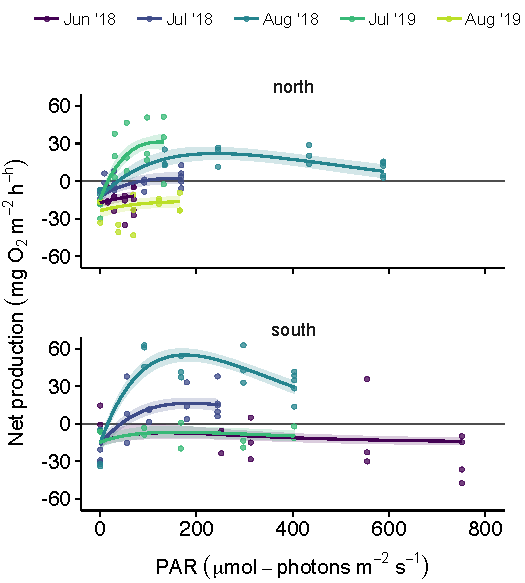
\includegraphics{../analysis/figures/fig_nep_pel.pdf}
\caption{\label{fig:nep-pel}
Fits of the photoinhibition curves to the pelagic data.
Ribbons are 68\% intervals matching nominal coverage of standard errors.
}
\end{figure}

\clearpage




% ---------------------------------------------------------------------------------------
% NEP - benthic
% ---------------------------------------------------------------------------------------

\begin{figure}
\centering
\linespread{1}
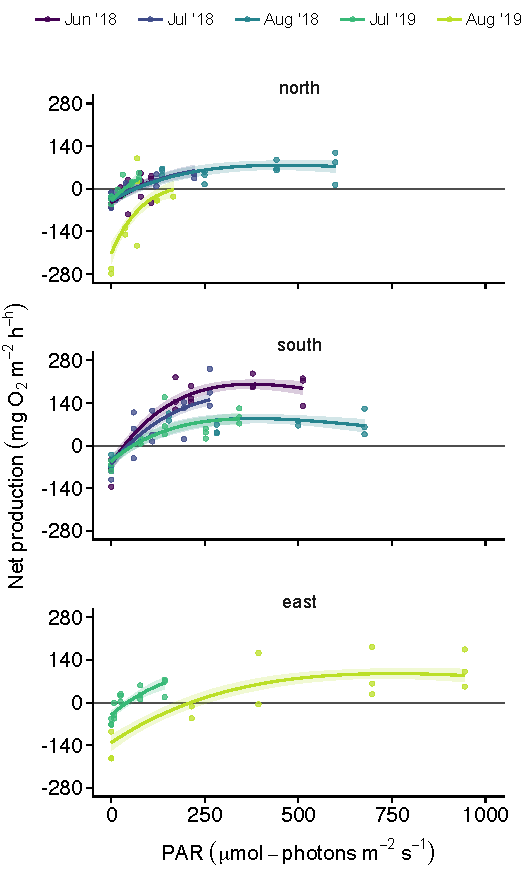
\includegraphics{../analysis/figures/fig_nep_ben.pdf}
\caption{\label{fig:nep-ben}
Fits of the photoinhibition curves to the benthic data.
Ribbons are 68\% intervals matching nominal coverage of standard errors.
}
\end{figure}

\clearpage

% ---------------------------------------------------------------------------------------
% PARS
% ---------------------------------------------------------------------------------------

\begin{figure}
\centering
\linespread{1}
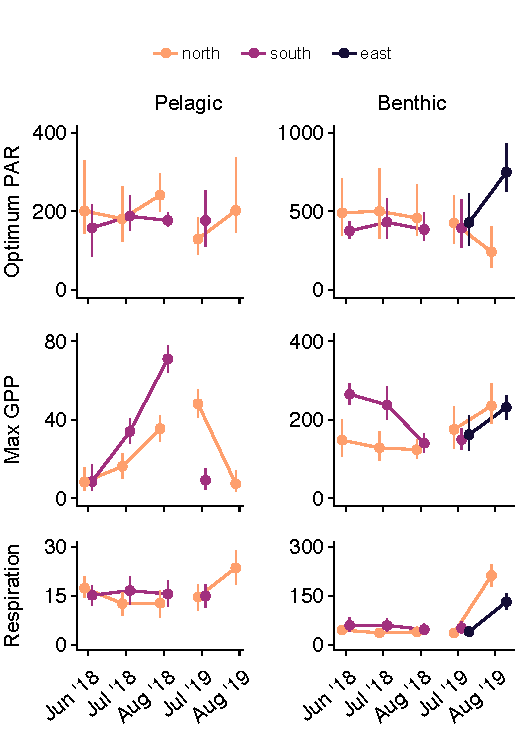
\includegraphics{../analysis/figures/fig_par.pdf}
\caption{\label{fig:par}
Variation in the metabolism parameters between sites and sampling dates.
max GPP and respiration are in units of $\text{mg}~\text{O}_2~\text{m}^{-2}~\text{h}^{-1}$
and optimum PAR is in units of $\mu\text{mol}~\text{photons}~\text{m}^{-2}~\text{s}^{-1}$.
Points are posterior medians 
and error bars are 68\% intervals matching nominal coverage of standard errors.
}
\end{figure}

\clearpage

% ---------------------------------------------------------------------------------------
% SD
% ---------------------------------------------------------------------------------------

\begin{figure}
\centering
\linespread{1}
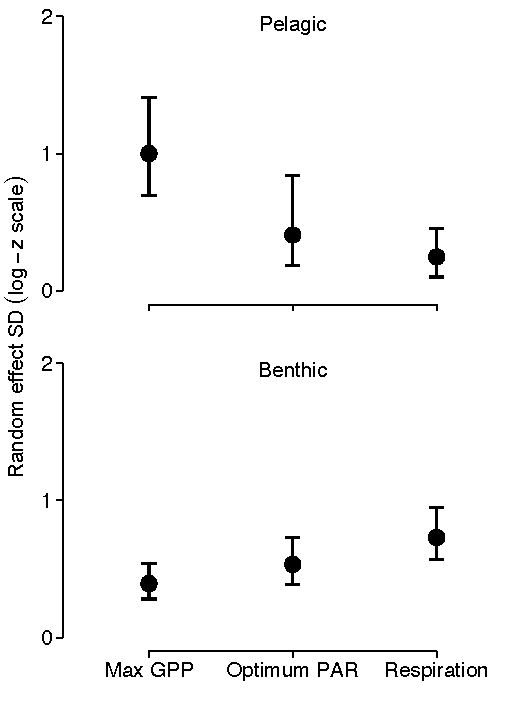
\includegraphics{../analysis/figures/fig_sd.pdf}
\caption{\label{fig:sd}
Standard deviations for variation in the metabolism parameters.
Points are posterior medians 
and error bars are 68\% intervals matching nominal coverage of standard errors.
}
\end{figure}

\clearpage

% ---------------------------------------------------------------------------------------
% VAR
% ---------------------------------------------------------------------------------------

\begin{figure}
\centering
\linespread{1}
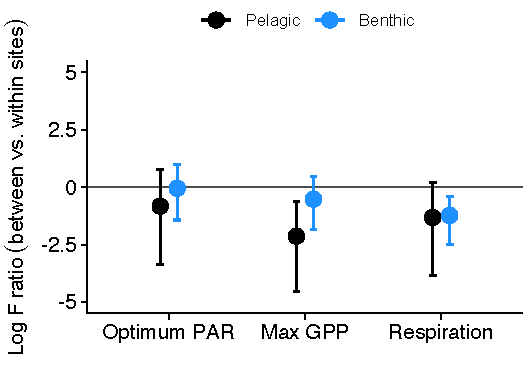
\includegraphics{../analysis/figures/fig_var.pdf}
\caption{\label{fig:var}
Log F ratios calculated from ANOVA for each parameter.
The ratio compares the variation between sites to the variation within,
and a log-ratio of 0 indicates equal variation. 
This was calculated over the full posterior distributions for each parameter;
the points are medians and 
and error bars are 68\% intervals matching nominal coverage of standard errors.
}
\end{figure}

\clearpage



% ---------------------------------------------------------------------------------------
% ---------------------------------------------------------------------------------------
% Supplement
% ---------------------------------------------------------------------------------------
% ---------------------------------------------------------------------------------------

\renewcommand{\thefigure}{S\arabic{figure}}
\renewcommand{\theequation}{S\arabic{equation}}
\renewcommand{\thetable}{S\arabic{table}}
\setcounter{equation}{0}
\setcounter{figure}{0}
\setcounter{table}{0}


\end{document}
